% ============================================== %

%%%%%%%%%%%%%%%%%%%%%%%%%%%%%%%%%%%%%%%%%%%%%%%%%%
%%%			  03 Trabalho Prático 03		   %%%
%%%%%%%%%%%%%%%%%%%%%%%%%%%%%%%%%%%%%%%%%%%%%%%%%%

% ============================================== %

\section*{Trabalho Prático 03}


Fazer os gráficos $P\times\delta_\mathrm{V}$, $P\times\delta_\mathrm{H}$, $P\times\theta$
para $\theta \in \left[0, \frac{\pi}{2}\right]$. Adotar:

$$
\left\{\begin{array}{lcl}
	k &=& 1000\text{ kN}\cdot\text{cm/rad} \\
	L &=& 100\:\:\text{cm} \\
	\Delta\theta &=& \frac{\pi}{36}\:\:\text{rad} \\
\end{array}\right.
$$

\begin{figure}[H]
	\centering
	\caption{Sistema estrutural do Trabalho Prático 3.}
	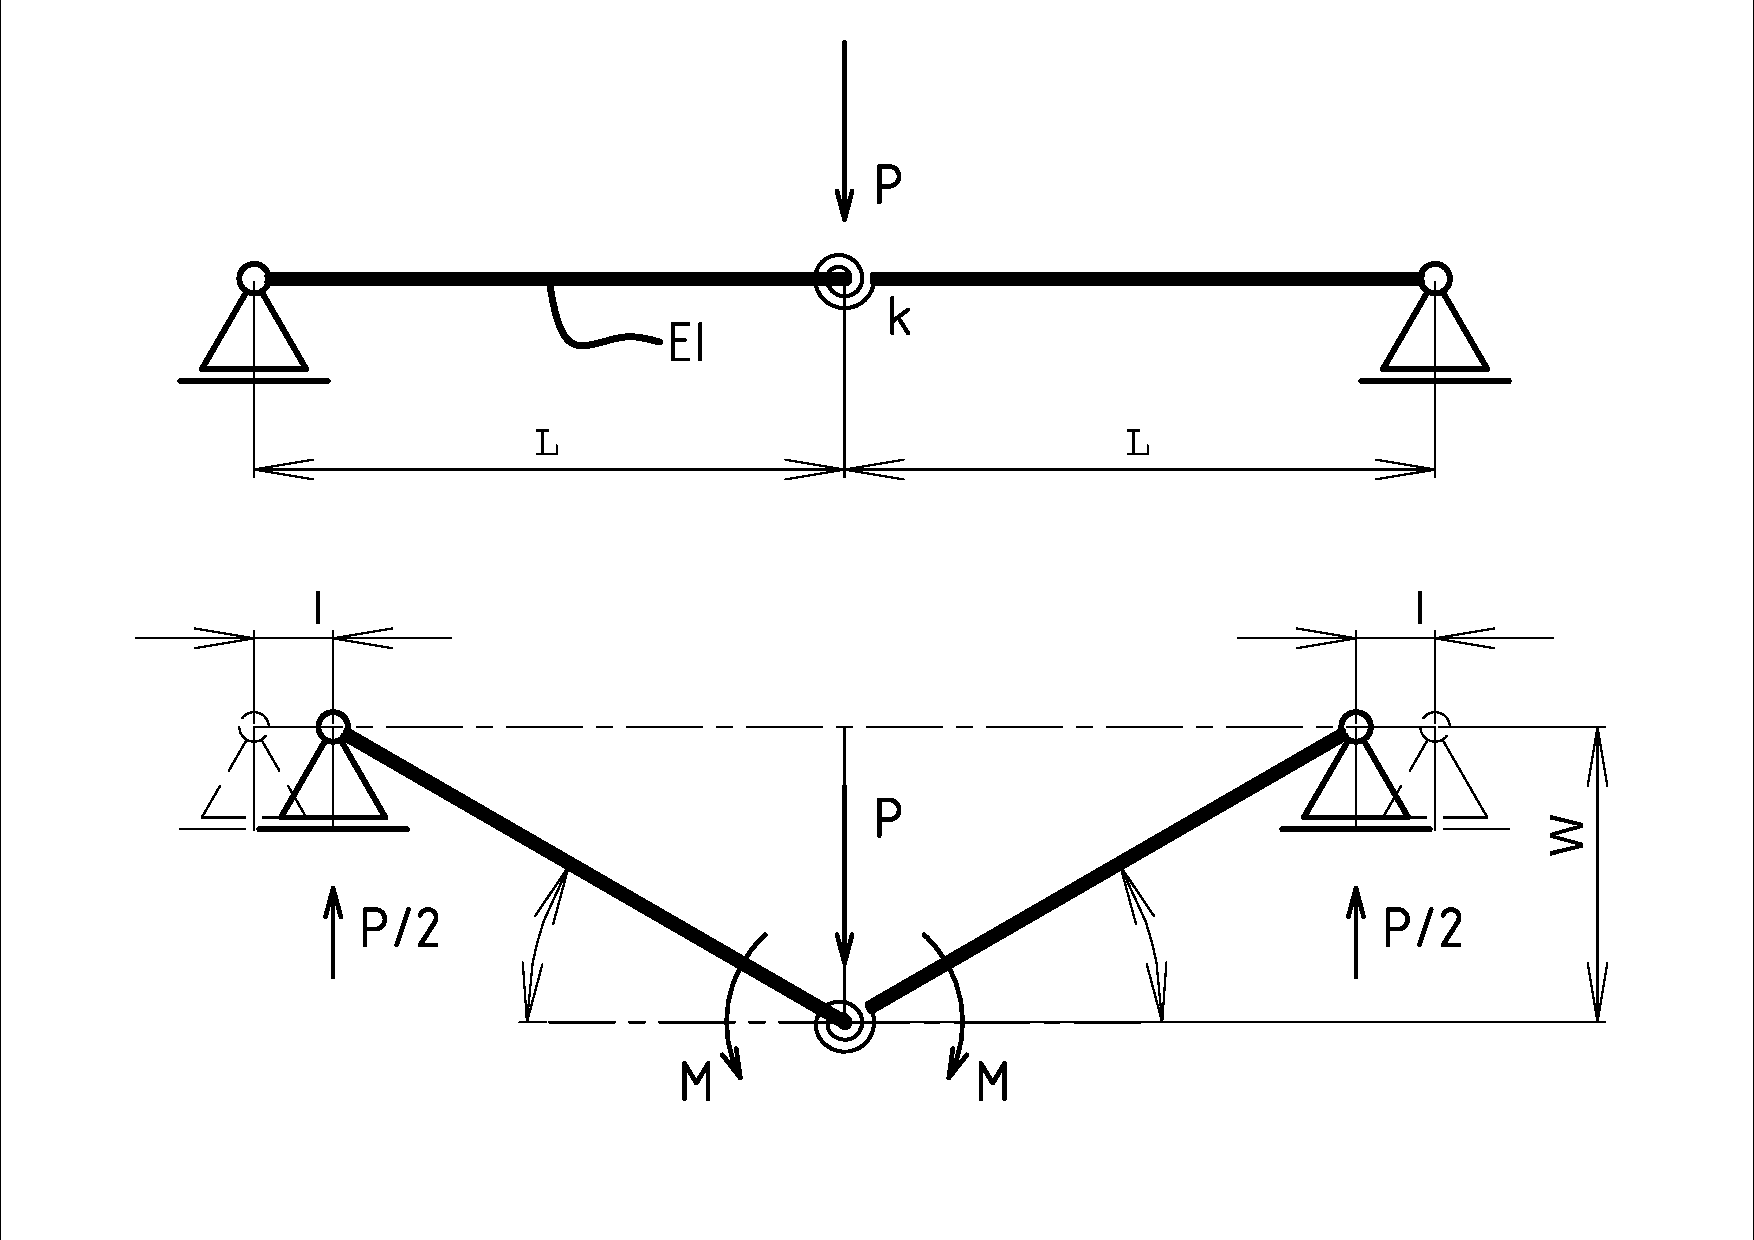
\includegraphics[
		trim=20mm 20mm 20mm 5mm,
		clip,
		width=\textwidth
	]{figuras/TPs-3.pdf}
\end{figure}


% ================ Resolução TP-03 ================
\begin{textocaixa}
\hspace{10mm}




\end{textocaixa}